%% ICAIF-style paper backbone for the CVaR-Constrained RL Portfolio Allocator.
%% Format intentionally mirrors recent ICAIF submissions (acmart, sigconf).
%% Numbers/figures are produced by the pipeline on the feat/cvar-allocator-pipeline
%% branch (scripts/run_diff_study.py, run_walk_forward.py, run_robustness.py,
%% run_ablations.py, run_macro_study.py; figures in paper/figures/).
%% Camera-ready (accepted, CMT ID 873): `anonymous` option removed.
\documentclass[sigconf]{acmart}

\usepackage{booktabs}
\usepackage{amsmath}
\usepackage{graphicx}
\usepackage{microtype}  % reduces overfull boxes via char protrusion / font expansion
\setlength{\emergencystretch}{3em}  % last-resort stretch to clear residual overfull lines
\setlength{\tabcolsep}{4.5pt}       % slightly tighter columns so wide tables fit the column
% Tighten float/caption spacing (content-neutral) to recover space for new
% analysis without cutting results; this paper carries an unusually high
% table density for an 8pp submission.
\setlength{\textfloatsep}{6pt plus 2pt minus 2pt}
\setlength{\floatsep}{4pt plus 2pt minus 2pt}
\setlength{\intextsep}{6pt plus 2pt minus 2pt}
\setlength{\abovecaptionskip}{3pt}
\setlength{\belowcaptionskip}{2pt}
\graphicspath{{figures/}}

\begin{document}

%% Rights block. ACM emails the exact commands after the eRights form is signed;
%% paste them over this block. Provisional values assume ACM Open (CC BY).
\setcopyright{cc}
\setcctype{by}
\acmConference[ICAIF '26]{7th ACM International Conference on AI in Finance}{November 14--17, 2026}{Milan, Italy}
\acmBooktitle{7th ACM International Conference on AI in Finance (ICAIF '26), November 14--17, 2026, Milan, Italy}
\acmYear{2026}
\copyrightyear{2026}
% \acmDOI{10.1145/XXXXXXX.XXXXXXX}   % TODO: from the ACM rights form
% \acmISBN{978-X-XXXX-XXXX-X/26/11}  % TODO: from the ACM rights form

\title{Making Tail Constraints Bind: Two Silent Failure Modes in
CVaR-Constrained Portfolio RL}

\author{Nigel Li}
\orcid{0009-0007-9869-3472}
\affiliation{%
  \institution{Columbia University}
  \city{New York City}
  \country{USA}}
\email{nl2992@columbia.edu}

\author{Yutong Han}
\orcid{0009-0004-0464-1398}
\affiliation{%
  \institution{Columbia University}
  \city{New York City}
  \country{USA}}
\email{yh3915@columbia.edu}

\begin{abstract}
A portfolio allocator trained by reinforcement learning (RL) to maximise return has no reason
to avoid large losses. The usual safeguard caps Conditional Value-at-Risk (CVaR), the average
loss in the worst weeks, through a Lagrangian penalty. We show that this safeguard can fail
silently in two ways. First, when the penalty and the reward sit on different scales, through
an unstandardised cost advantage or a dual step mis-scaled to the CVaR excess, the penalty
weight stays at zero and the budget is never enforced, even as tail metrics keep improving.
Second, the evaluation protocol can decide the winner. On a broad cross-asset universe, a single stress window ranks the learned allocator above every classical optimiser, a rolling
walk-forward reverses that ranking, and the reduction in tail risk holds under both. Plotting the multiplier during training exposes
the first failure, and rolling out-of-sample folds expose the second. Fixing
the scale makes the penalty bind in training, but the budget is still breached in most
out-of-sample weeks. We therefore add a decision-time filter. Before each trade, it forecasts
the portfolio's CVaR from trailing data and, when the forecast exceeds the budget, moves the
portfolio toward minimum variance. At matched settings, the filter cuts the breach rate from
$75.1\%$ to $7.4\%$, close to the classical optimisers, at a Sharpe ratio comparable to rolling
minimum variance. Across a rolling walk-forward on two ETF universes with weekly data and
trading costs, the reduction in tail risk is statistically significant, including when folds
are clustered by calendar and after Benjamini--Hochberg control. What the constraint delivers
is protection against deep losses, and that protection survives multiple-testing correction.
\end{abstract}

\begin{CCSXML}
<ccs2012>
<concept><concept_id>10010147.10010257.10010258.10010261</concept_id>
<concept_desc>Computing methodologies~Reinforcement learning</concept_desc>
<concept_significance>500</concept_significance></concept>
<concept><concept_id>10010405.10010455.10010460</concept_id>
<concept_desc>Applied computing~Economics</concept_desc>
<concept_significance>300</concept_significance></concept>
</ccs2012>
\end{CCSXML}
\ccsdesc[500]{Computing methodologies~Reinforcement learning}
\ccsdesc[300]{Applied computing~Economics}

\keywords{portfolio allocation, reinforcement learning, Conditional
Value-at-Risk, drawdown control, constrained MDP, differentiable optimisation}

\maketitle

%% =====================================================================
\section{Introduction}

A portfolio allocator decides, each week, how to split capital across assets. Reinforcement
learning (RL) can learn such a rule from data, but a rule trained only to earn return has no
reason to limit its worst losses. In the week of 16 March 2020 the S\&P 500 fell about 15\%
over five sessions and the VIX closed at a record 82.69. An allocator trained without a loss
limit kept holding equities, whereas an otherwise identical allocator with one had already
rotated into Treasuries and cash before the trough, and lost about half as much. Its drawdown was 7.7\% in March 2020 against 16.3\%, and 11.8\% against 20.6\% over the whole 2020--2024 window (Figure~\ref{fig:stress_paths}, Table~\ref{tab:stress}).

\begin{figure}[t]
  \centering
  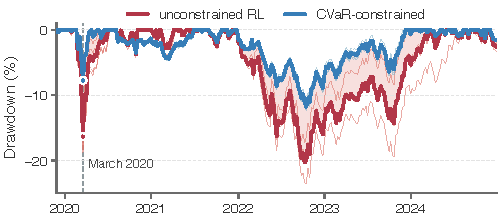
\includegraphics[width=\columnwidth]{figure_stress_paths.pdf}
  \Description{Line chart of drawdown from 2020 to 2024. The CVaR-constrained allocator's drawdown is about half the unconstrained allocator's in both the March 2020 crash and the 2022 selloff.}
  \caption{Drawdown on the 2020--2024 stress window. Thick lines follow the five-seed mean return path and thin lines the individual seeds.}
  \label{fig:stress_paths}
\end{figure}

The limit we use is Conditional Value-at-Risk (CVaR), the average loss over the worst few
percent of weeks~\cite{rockafellar2000optimization}. The standard way to impose such a limit in
RL is a Lagrangian penalty~\cite{altman1999cmdp}, in which the learner pays a price $\lambda$ for each
unit of CVaR above its budget, and $\lambda$ rises automatically while the budget is
exceeded. We show two ways in which this machinery can appear to work while the limit is never
enforced.\looseness=-1

\paragraph{Failure 1. The penalty never switches on} If the penalty signal is on a much smaller
scale than the reward signal, $\lambda$ stays near zero and the budget exists only on paper.
Safe-RL work already knows that $\lambda$ responds slowly and depends on its step
size~\cite{stooke2020pid}, and libraries such as OmniSafe standardise the cost signal by
default~\cite{ji2024omnisafe}. In portfolio allocation the failure is easy to miss, because
the raw cost signal is $O(10^{-3})$ against a unit-scale reward, and because tail metrics improve anyway through other parts of the pipeline. The problem only shows
up if one plots $\lambda$ over training (Section~\ref{sec:coupling}).

\paragraph{Failure 2. The test protocol picks the winner} Finance has long known that
optimised portfolios which look strong in one sample often fail out of
sample~\cite{demiguel2009optimal,bailey2014deflated}, but RL portfolio studies usually report a
single test window. On a 31-asset universe, one stress window ranks our learned allocator above
every classical optimiser, while a 20-fold rolling walk-forward reverses that ranking
(Section~\ref{sec:protocol}). ``Beat-the-optimiser'' results can therefore be artefacts of the
split.

\paragraph{The fix} Even a correctly scaled penalty only discourages breaches on average, so
the budget is still breached out of sample. We therefore check every proposed portfolio before
it trades, in the manner of a safe-RL safety layer~\cite{dalal2018safe}. If its estimated forward CVaR exceeds the budget, the portfolio is shrunk toward a minimum-variance portfolio
until it complies.

\paragraph{Contributions}
\begin{enumerate}
\item Two named failure modes, with diagnostics and fixes. The first is a \emph{Lagrangian constraint-coupling failure}, wherein a scale mismatch between the reward and constraint
channels leaves $\lambda$ inert, through an unstandardised cost advantage in a model-free
actor--critic and through a dual step mis-scaled to the CVaR excess in a differentiable
allocator (Section~\ref{sec:coupling}). The second is an \emph{evaluation-protocol reversal} between a
single stress window and a rolling walk-forward (Section~\ref{sec:protocol}).
\item A differentiable CVaR-constrained allocator whose tail effect survives
multiplicity control. A return objective plus a differentiable CVaR penalty is
back-propagated through the rollout of a leak-free, tested environment
(Section~\ref{sec:method}), and the decision-time filter cuts out-of-sample breach from
$75.1\%$ to $7.4\%$ at matched dual settings. The tail-risk reduction holds on a 40-fold,
two-universe walk-forward under Benjamini--Hochberg and (for Sharpe) Deflated-Sharpe
control (Section~\ref{sec:significance}), and a regime-switching hybrid reaches a walk-forward Sharpe
of $1.316$ vs $1.209$ for pure minimum variance, with overlapping bootstrap intervals
(Table~\ref{tab:hybrid}).
\item An evaluation protocol built to expose this kind of artefact. Deterministic
optimisers and three tuned model-free RL families are compared under a two-universe rolling
walk-forward with Wilcoxon, Benjamini--Hochberg and Deflated-Sharpe control, which is what
surfaces the reversal in Contribution~1.
\end{enumerate}

Our central claim is that the constraint protects against deep losses. We contribute a constraint that measurably
binds and lowers tail losses, a decision-time filter that keeps a learned policy within its
budget out of sample, and two failure modes that other studies of constrained RL in finance
can check for.\looseness=-1

%% =====================================================================
\section{Background and related work}
\label{sec:related}

\paragraph{Mean--variance optimisation and its inputs} Mean--variance optimisation
(MVO)~\cite{markowitz1952portfolio} is sensitive to input estimates. Decision-focused
learning trains return predictors to improve downstream MVO decisions rather than raw forecast
accuracy~\cite{lee2024dfl}, and mean--variance-efficient collaborative filtering
blends user preference with portfolio theory~\cite{chung2023mvecf}. Both improve the
inputs to a variance-based objective. We instead constrain a tail risk
measure on a learned policy.\looseness=-1

\paragraph{Conditional Value-at-Risk} $\mathrm{CVaR}_\alpha$ is the expected
portfolio loss on the worst $(1{-}\alpha)$ fraction of outcomes, the average of losses
exceeding the $\alpha$-quantile ($\mathrm{VaR}_\alpha$). Unlike variance, it ignores the
upside, and unlike $\mathrm{VaR}$, it averages across the whole tail. Rockafellar and
Uryasev~\cite{rockafellar2000optimization} give the tractable form
\begin{equation}\label{eq:ru}
  \mathrm{CVaR}_\alpha(L) \;=\; \min_{\zeta\in\mathbb{R}}\!\left\{
    \zeta + \frac{1}{1-\alpha}\,\mathbb{E}\!\left[\max(L-\zeta,\,0)\right]
  \right\},
\end{equation}
where $L$ denotes the portfolio loss and the inner expectation is over the empirical
loss distribution. The minimum in~\eqref{eq:ru} is attained at $\zeta=\mathrm{VaR}_\alpha$, and the
representation admits both a convex linear program (LP), included as a baseline, and a
differentiable penalty via \texttt{topk}.\looseness=-1

\paragraph{RL for portfolio management}
Most RL portfolio papers train on a single historical window, test on one held-out split,
and compare against equal weight or buy-and-hold. EIIE~\cite{jiang2017deep} compares twelve classical strategies on three
$\approx$50-day crypto back-tests, and SARL~\cite{ye2020sarl} reports higher return on a fixed
period without cross-validation. FinRL~\cite{liu2021finrl} supports rolling retraining but
demonstrates it on a single split with no significance tests. Huang~\cite{huang2025ctrl}
applies continuous-time RL to asset--liability management, although with a quadratic
surplus objective rather than a tail constraint. None of these uses CVaR as a constraint,
seeds multiple runs, or applies statistical testing. Empirical finance has long documented
how the selection of backtests inflates reported
performance~\cite{white2000reality,harvey2016cross,bailey2017pbo} and that optimised portfolios
rarely beat naive ones out of sample~\cite{demiguel2009optimal}, and our protocol carries
those controls over to RL portfolio allocation. We are not aware of prior work that subjects
RL portfolio allocation to a 40-fold, two-universe walk-forward with Wilcoxon and
Benjamini--Hochberg control, which is the protocol that exposes the reversal artefact.

\paragraph{Direct reinforcement and pathwise gradients}
Moody and Saffell~\cite{moody2001learning} trained a recurrent trading policy by
back-propagating the \emph{differential Sharpe ratio} directly through the return
function. Buehler et al.~\cite{buehler2019deephedging} (Deep Hedging) extend this to
neural derivative hedging, back-propagating CVaR as a risk-aversion \emph{utility}
through a simulated trajectory. Our allocator uses the same pathwise gradients, but replaces
the risk-aversion coefficient with an explicit CVaR
\emph{budget constraint} enforced by a dual variable. Model-free policy gradients
(Advantage Actor-Critic, A2C, and Proximal Policy Optimization,
PPO~\cite{schulman2017ppo}) and off-policy actor--critics
(Soft Actor-Critic, SAC~\cite{haarnoja2018soft}) ignore this differentiable structure. Our allocator
exploits it, which matters at this sample size (887 weekly observations,
Section~\ref{sec:modelfree}). ProtoHedge~\cite{faloughi2025protohedge} similarly makes
such policies auditable via a prototype-similarity policy.

\paragraph{CVaR-constrained RL}
Chow et al.~\cite{chow2018riskconstrained} derive the Lagrangian gradient for CVaR-constrained
CMDPs. Tessler et al.~\cite{tessler2019rcpo} (RCPO) impose general constraints by a
Lagrangian penalty and Ying et al.~\cite{ying2022cppo} (CPPO) constrain CVaR, both in robotics. Lagrange multipliers are known to
respond slowly and to depend on their step size~\cite{stooke2020pid}, and safe-RL libraries
standardise the cost advantage by default~\cite{ji2024omnisafe}. None of this work documents
the resulting \emph{constraint-coupling failure} in portfolio allocation. There the raw CVaR
cost is $O(10^{-3})$ against a unit-scale reward advantage, a mismatch that robotics benchmarks
would not expose. We pose allocation as a constrained MDP~\cite{altman1999cmdp,achiam2017cpo} and show that a
well-scaled dual is what makes the constraint bind. The closest concurrent work is
\citet{dong2025clauselens} (\textsc{ClauseLens}), a CVaR-constrained RL system for
reinsurance pricing. Our work is complementary, since the failure modes we describe apply to
any CVaR-constrained financial RL system.

%% =====================================================================
\section{Problem formulation}
\label{sec:formulation}

\paragraph{Markov Decision Process (MDP)} Each week $t$, the agent observes a state $s_t$ and chooses
post-trade weights $w_t$ on the long-only simplex. The state holds each asset's 26-week momentum
and volatility, the current weights, the drawdown, a rolling 95\% CVaR estimate and, optionally,
exogenous macro and factor features. The environment projects $w_t$ onto the admissible set
$\mathcal{W}$ (max weight 0.40, turnover cap 0.50, optional cash floor), charges a proportional
cost $c\lVert w_t - w_{t-1}\rVert_1$ with $c=5$\,bps, and realises the net return
$r_t = w_t^{\top}\rho_t - c\lVert w_t - w_{t-1}\rVert_1$, where $\rho_t$ are next-week asset
returns. Features at $t$ use only $\rho_{<t}$ (no look-ahead, enforced by
tests).\looseness=-1

\paragraph{Constrained objective (CMDP)} A \emph{constrained Markov Decision
Process} (CMDP)~\cite{altman1999cmdp} adds to the MDP one or more inequality constraints that
the policy must satisfy on average. We maximise risk-adjusted return subject to a tail budget,
$\max_\pi J(\pi)$ s.t.\ $\mathrm{CVaR}_\alpha(\text{loss})\le d$ with $\alpha=0.95$. The
Lagrangian relaxation turns the constraint into a penalty, $\mathcal{L}(\pi,\lambda)=J(\pi) -
\lambda\,(\mathrm{CVaR}_\alpha - d)$. The dual variable $\lambda\ge0$ (the \emph{dual}, or
multiplier) is raised whenever the constraint is violated and lowered when slack remains. In
equilibrium, $\lambda$ is the shadow price of tail risk, so a higher $\lambda$ means that the
policy has been pushing against its tail budget. A portfolio is \emph{over budget} when its
$\mathrm{CVaR}_{0.95}$ (the mean weekly loss in its worst 5\% of weeks) exceeds $d$ ($1.2\%$ unless stated). It is measured on the sampled window in training, on the trailing 52 realised weeks at test time, and
on a trailing forecast in the filter. The \emph{breach rate} is the share of test weeks over
budget (5\% tolerated). We mostly report $\mathrm{CVaR}_{0.99}$, a deeper tail than the one
constrained and so a stricter test. CVaR and drawdowns are fractions of wealth.\looseness=-1

%% =====================================================================
\section{Method}
\label{sec:method}

\paragraph{Differentiable allocator} The actor is an MLP mapping $s_t$ to simplex
weights via softmax. The environment's reward and a sample CVaR are both differentiable in $w$,
so over randomised training windows we back-propagate the objective
\begin{equation}\label{eq:loss}
\mathcal{L} = -\,\mathrm{Sharpe}(\text{net returns})
  \;+\; \lambda\,\mathrm{ReLU}(\widehat{\mathrm{CVaR}} - d)
  \;+\; \kappa\,\text{turnover}.
\end{equation}
Here $\mathrm{Sharpe}=\bar{r}/\sigma_r$ is the window's mean net return divided by its
standard deviation (reward per unit of risk), $\widehat{\mathrm{CVaR}}$ is the mean
tail loss over the worst $(1{-}\alpha)$ fraction of window net returns (a differentiable
tail mean via \texttt{topk}), and $d$ is the pre-specified tail budget. This \emph{pathwise} gradient,
taken through the portfolio return itself, needs far fewer samples than \emph{score-function} RL
(PPO, A2C), which estimates it from sampled actions (Section~\ref{sec:modelfree}).

\paragraph{Pathwise gradient and where the constraint acts} Because every term in
$\mathcal{L}$~\eqref{eq:loss} is a differentiable function of the rollout, the policy is trained
by exact back-propagation through the simplex map and the reward, without a
score-function estimator. With net returns $r_t = w_t^{\top}\rho_t - c\lVert w_t-w_{t-1}\rVert_1$
and tail set $\mathcal{T}=\{t \mid r_t \text{ among the worst } \lceil(1-\alpha)T\rceil
\text{ of the window}\}$, the gradient is
\begin{equation}\label{eq:grad}
\frac{\partial \mathcal{L}}{\partial \theta}
= \sum_{t}\Big(
  \underbrace{-\tfrac{\partial\,\mathrm{Sharpe}}{\partial r_t}}_{\text{all weeks}}
  \;-\;
  \underbrace{\tfrac{\lambda}{|\mathcal{T}|}\,
  \mathbf{1}[\widehat{\mathrm{CVaR}}>d]\,\mathbf{1}[t\in\mathcal{T}]}_{\text{tail weeks only}}
  \Big)\,\frac{\partial r_t}{\partial w_t}\,\frac{\partial w_t}{\partial \theta},
\end{equation}
where $\partial w_t/\partial\theta$ flows through the residual softmax
(below). The \texttt{topk} subgradient in~\eqref{eq:grad} sends the dual pressure to exactly the
worst-$(1-\alpha)$ weeks, and only while the constraint is breached. The penalty therefore
pushes up the worst weeks and leaves the rest of the path largely alone, so the constraint binds once the dual is correctly scaled (Section~\ref{sec:coupling}).

\paragraph{Residual policy over an adaptive anchor} To generalise across regimes
rather than overfit one price path, the weights are $w_t = \mathrm{softmax}(\log a_t +
f_\theta(s_t))$, where $a_t$ is an adaptive inverse-volatility anchor computed from
recent returns. At initialisation $f_\theta \approx 0$, so the policy starts as the anchor, a regime-robust prior, and training then learns a state-dependent tilt. Two choices curb backtest overfitting. Model selection keeps the checkpoint with the best validation
objective among those that satisfy the validation CVaR limit, and weight decay is applied.

\paragraph{Baselines} The deterministic baselines are cash, equal weight, inverse
volatility, minimum variance, mean--variance, risk parity and a min-CVaR
Rockafellar--Uryasev LP~\cite{rockafellar2000optimization}, all re-estimated weekly. The
covariance-based rules use the sample covariance of the trailing 104 weeks, and inverse
volatility the trailing 52 weeks, and all are long-only under the learner's weight cap. Within each
evaluation window, they are re-estimated from that window's returns, with a minimum of 26 weeks
of history (equal weight before that). The learned baselines are model-free A2C,
PPO~\cite{schulman2017ppo} (clipped surrogate, generalised advantage estimation, GAE), SAC~\cite{haarnoja2018soft}
(off-policy, twin critics, auto-tuned entropy), and the unconstrained differentiable allocator ($\lambda=0$).\looseness=-1

\paragraph{Regime-switching hybrid}
We build a hybrid that needs no retraining. Each out-of-sample (OOS) week is labelled
\emph{high-volatility} if trailing 13-week SPY volatility meets the 75th-percentile cutoff (15\%
of OOS weeks), \emph{selloff} if cumulative return is $\le -5\%$, and \emph{calm} otherwise. The
hybrid applies constrained RL in high-volatility weeks and rolling minimum variance otherwise,
reusing the existing OOS paths without refitting. On the 26-week macro walk-forward, this labels
80 of 520 weeks as high-volatility, and in those weeks constrained RL has Sharpe $1.415$ against
$0.564$ for minimum variance (Table~\ref{tab:hybrid}). These labels differ from the regime split
in Table~\ref{tab:regime}.\looseness=-1

\emph{Threshold sensitivity.} The switch depends on two labelling thresholds, so
we sweep them over $\text{vol-quantile}\in\{0.65,\dots,0.85\}$ and $\text{selloff}\in\{-0.04,-0.05,-0.06\}$, giving 15 configurations with no retraining (Table~\ref{tab:threshold}).
The hybrid beats pure minimum variance in 10 of 15 configurations, with a mean gain of
$+0.077$. It wins at every volatility cutoff when the selloff threshold is $-0.04$
or $-0.05$, but loses at all five cutoffs once the threshold deepens to $-0.06$. That threshold
relabels as selloffs the high-volatility weeks in which the constrained allocator adds most,
and routes them to minimum variance instead. The default $(0.75,-0.05)$, fixed before the
sweep, gives $+0.107$, and seven of the ten winning configurations give a larger gain.

\begin{table}[t]
\centering
\caption{Sharpe gain of the hybrid over minimum variance across 15 threshold settings, with no retraining. The default is $(0.75,-0.05)$.}
\label{tab:threshold}
\footnotesize
\setlength{\tabcolsep}{4pt}
\begin{tabular}{@{}lrrrrr@{}}
\toprule
selloff \textbackslash{} vol.\ quantile & 0.65 & 0.70 & 0.75 & 0.80 & 0.85 \\
\midrule
$-0.04$ & $+0.202$ & $+0.230$ & $+0.161$ & $+0.225$ & $+0.058$ \\
$-0.05$ & $+0.154$ & $+0.179$ & $+0.107$ & $+0.169$ & $+0.002$ \\
$-0.06$ & $-0.007$ & $-0.017$ & $-0.086$ & $-0.034$ & $-0.183$ \\
\bottomrule
\end{tabular}
\end{table}

%% =====================================================================
\section{Decomposing the constraint into the dual, the architecture and budget feasibility}
\label{sec:coupling}

This section asks what the Lagrangian penalty contributes. It reports three findings, then the filter that addresses the third. We compare four versions, or
\emph{arms}, of the differentiable allocator (Table~\ref{tab:coupling}, top block). They are A1 unconstrained, A2 mis-scaled dual, A3 scaled dual, and A4, the scaled dual with a loose budget.
All four share the residual actor, weight projection and budget (5 seeds, 1500 updates), and A2--A4 also share the CVaR penalty and CVaR-limited checkpoint selection. A2 and A3 differ only in the
dual step, and A4 differs from A3 only in $d$. The mis-scaled dual updates $\lambda$ with step $\eta_\lambda=0.001$, far too small for the size of the CVaR excess, while the scaled dual uses $\eta_\lambda=5.0$, which matches it. The unconstrained
arm drops the penalty and selects checkpoints on validation return alone. The stress window
trains on 2008--2018 and tests from late 2019 to 2024. Here the \emph{rolling breach rate} is
the share of test weeks in which the rolling 52-week $\mathrm{CVaR}_{0.95}$ exceeds the training
budget $d$, so a rate of 1.000 means over budget in every test week.\looseness=-1

\paragraph{Finding 1. A scale mismatch leaves the dual inert} With the mis-scaled dual (A2),
$\lambda$ stays near zero throughout training (Figure~\ref{fig:lambda}), with a mean final value of $0.022$ against $0.101$ for the scaled dual (A3). The dual update is
$\lambda \leftarrow \max\{0,\ \lambda + \eta_\lambda(\widehat{\mathrm{CVaR}} - d)\}$, and the CVaR
excess is about $10^{-2}$ in weekly-return units, so with a step of $10^{-3}$ each update moves
$\lambda$ by roughly $10^{-5}$, and 1500 updates are not enough. The model-free actor--critic
failed in the same way, through its \emph{advantages} (how much better an action did
than the critic expected). Its reward advantage was standardised to unit scale while its cost advantage stayed at about $10^{-3}$, so the constrained and unconstrained
agents trained identically. After we standardised the cost advantage and drove the dual with a
breach indicator, $\lambda$ rose to $O(1)$. As a check, if $\lambda$ stays at zero throughout training, the constraint has no effect, whatever the loss curve looks like.\looseness=-1

\begin{figure}[t]
  \centering
  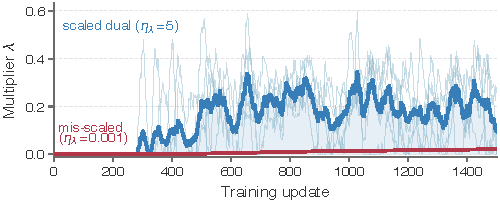
\includegraphics[width=\columnwidth]{figure_lambda_trace.pdf}
  \Description{Line chart of the Lagrange multiplier over 1500 training updates. The mis-scaled dual stays near zero throughout, while the scaled dual rises to between 0.1 and 0.3 after a few hundred updates.}
  \caption{The Lagrange multiplier over training. Thick lines are five-seed means and thin lines the individual seeds. $\lambda$ is zero while the anchor-initialised policy meets $d$.}
  \label{fig:lambda}
\end{figure}

\paragraph{Finding 2. Most of the tail control comes from the pipeline} Most of the tail
reduction does not depend on the penalty. Even with $\lambda$ close to zero, the constrained
pipeline lowers CVaR$_{99}$ by $61\%$ relative to the unconstrained learner ($0.025$ vs $0.065$,
5-seed mean) and raises Sharpe by $58\%$ ($0.987$ vs $0.626$). The reduction comes from checkpoint
selection under the CVaR limit, on top of the shared anchor and projection. A permutation test
on the 5-seed distributions confirms the difference (observed $-0.039$, one-sided $p=0.0044$,
two-sided $p=0.0083$, $n=50{,}000$), and the scaled dual gives a similar reduction ($p=0.0037$).
Engaging the dual properly ($\lambda=O(0.1)$) barely changes CVaR$_{99}$ ($0.028$ vs $0.025$), so
most of the $61\%$ comes from the pipeline. The pipeline thus controls the tail without help
from the penalty, which also explains why the coupling failure goes unnoticed. Tail metrics improve whether or not the dual works, and only the trace of the multiplier shows
that it is inactive.\looseness=-1

\paragraph{Finding 3. Meeting the budget out of sample is a separate problem} Scaling the
dual fixes training but not the test window. The scaled dual binds in training, but at the tight
budget ($d=1.2\%$) it breaches more often out of sample than the mis-scaled dual ($75\%$ of test
weeks against $8\%$), although classical rules meet the same budget in $92\%$ of weeks
(Section~\ref{sec:budget-reach}). It is worse than the mis-scaled dual on every metric in
Table~\ref{tab:coupling}.\looseness=-1

Checkpoint selection explains why. With the dual scaled, most checkpoints meet the validation
budget (27 of 30 on average, against 8 of 30), so selection keeps a later checkpoint that leans
further toward return (update 1010 on average, against 370), and that checkpoint breaches when
the tail shifts in the test window. Changing $d$ does not fix this. Four rules for setting $d$
from validation data, fixed in advance, all give $71$--$78\%$ out-of-sample breach. They are a loose $1.92\%$ budget (A4), the policy's own or the anchor's validation $\mathrm{CVaR}_{0.95}$, and a
per-fold adaptive budget over a 10-fold walk-forward. Whatever the value of $d$, a Lagrangian
learner whose dual binds gives up compliance when the tail shifts, so the remedy has to act on
the portfolio itself.\looseness=-1

\paragraph{The fix is a decision-time filter} We therefore enforce the budget at the moment of
trading with a CVaR \emph{filter}, a safety layer in the sense of~\citet{dalal2018safe} that sits
between the actor and the environment. For each proposed portfolio, it estimates forward CVaR
from the trailing mean $\mu_p$ and volatility $\sigma_p$ as $\mathrm{CVaR}\approx
c_\alpha\sigma_p-\mu_p$, where $c_\alpha=\varphi(\Phi^{-1}(\alpha))/(1-\alpha)$ is the Gaussian
CVaR multiplier ($c_{0.95}=2.06$). If the estimate exceeds $d$, the filter moves the proposal
along the line toward a trailing minimum-variance portfolio, using the largest mixing weight
that clears the budget. The turnover, max-weight and long-only limits then apply as before. We
train with the filter on.\looseness=-1

The filter uses no future data. The trailing mean, covariance and minimum-variance anchor come
from the $L=104$ returns $\rho_{t-L},\dots,\rho_{t-1}$, and the actor's features use only
$\rho_{<t}$, so the decision at $t$ depends only on $\mathcal{F}_{t-1}$. An automated look-ahead
test confirms that shifting the return series leaves the decision at $t$ unchanged, with zero
deviation.\looseness=-1

Four further arms, A5--A8, match the coupling arms exactly (5 seeds, 1500 updates, same splits) and change
only the named quantities (Table~\ref{tab:coupling}, bottom block, and Figure~\ref{fig:frontier}).
A6, the method we propose, adds the filter to the scaled dual. At the same $\eta_\lambda$, it
lowers breach from $75.1\%$ to $7.4\%$, below every classical rule, with $\mathrm{CVaR}_{99}$
$0.016$, mean excess $0.0043$ and Sharpe $0.851$. A5 adds the filter to the mis-scaled dual
($\eta_\lambda=0.001$) and matches the mis-scaled row. That policy already sits within budget,
so the filter never triggers (0 of 1285 test weeks across seeds). A5 reaches the classical
$7.9\%$ at Sharpe $0.987$, against $0.901$ for minimum variance, with breaches less than half as
deep (mean excess $0.0126$ vs $0.0294$). A7 is the negative control, which updates $\lambda$ online from realised losses with the filter off. Its breach rate stays at $81.9\%$ even as $\lambda$
climbs to a mean of $7.69$, so adjusting the dual at test time does not enforce the budget, and
the improvement in A6 is due to the filter. A8 pairs the filter with the adaptive dual and
recovers most of the compliance ($14.6\%$), though less reliably, ranging from $7$ to $33\%$ across seeds,
whereas A5 and A6 do not vary between seeds.\looseness=-1

The filtered arms hold low-volatility portfolios that differ measurably from minimum variance. A5's weights are a mean $L_1$ distance of $0.476$ from rolling minimum variance, with
correlation $0.786$ and a different top holding in $9.4\%$ of rebalances, against $0.890$,
$0.201$ and $97.5\%$ for the unfiltered scaled dual. In that region, A5 beats minimum variance on
both axes, with higher Sharpe at an equal breach rate and half the breach depth, and A6 has a
lower breach rate. Out of sample, the scaled soft penalty did not keep the portfolio within
budget, and the decision-time projection (A6) did.

\begin{table}[t]
\centering
\caption{Coupling ablation and decision-time filter on the stress window (5-seed means). $^\dagger$Mean online-updated $\lambda$ at evaluation.}
\label{tab:coupling}
\footnotesize
\setlength{\tabcolsep}{4pt}
\begin{tabular}{@{}lrrrr@{}}
\toprule
variant & Sharpe & CVaR$_{99}$ & breach rate & final $\lambda$ \\
\midrule
A1 unconstrained & $0.626$ & $0.065$ & $1.000$ & $0.000$ \\
A2 mis-scaled dual ($\eta_\lambda{=}0.001$) & $0.987$ & $0.025$ & $0.079$ & $0.022$ \\
A3 scaled dual ($\eta_\lambda{=}5.0$, $d{=}1.2\%$) & $0.911$ & $0.028$ & $0.751$ & $0.101$ \\
A4 scaled dual, loose ($d{=}1.92\%$) & $0.543$ & $0.050$ & $0.780$ & $0.046$ \\
\midrule
A5 filter only ($\eta_\lambda=0.001$) & $0.987$ & $0.025$ & $0.079$ & $0.003$ \\
A6 filter + scaled dual ($\eta_\lambda=5.0$) & $0.851$ & $0.016$ & $0.074$ & $0.135$ \\
A7 adaptive dual ($\eta_\lambda=5.0$ online) & $0.826$ & $0.031$ & $0.819$ & $7.692^\dagger$ \\
A8 filter + adaptive dual & $0.800$ & $0.020$ & $0.146$ & $0.657^\dagger$ \\
\bottomrule
\end{tabular}
\end{table}

\begin{figure}[t]
  \centering
  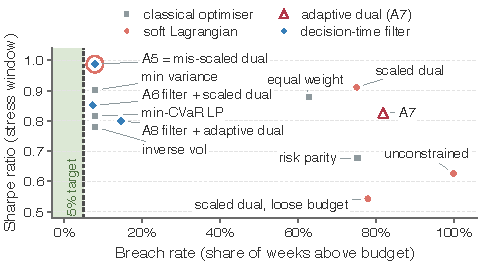
\includegraphics[width=\columnwidth]{figure_filter_frontier.pdf}
  \Description{Scatter plot of Sharpe ratio against breach rate. Classical optimisers and the filtered arms cluster near the 5 percent target line at Sharpe 0.8 to 1.0, while the soft Lagrangian arms and the adaptive dual without the filter lie at breach rates of 60 to 100 percent.}
  \caption{Breach rate against Sharpe on the stress window. The dashed line marks the 5\% tolerated breach rate. Squares are classical optimisers, diamonds the filtered arms (A5, A6, A8), circles A1--A4 and the triangle the adaptive dual without the filter (A7). The ringed point is the mis-scaled dual, which A5 overlaps.}
  \label{fig:frontier}
\end{figure}

\paragraph{Is the budget infeasible, or is the policy failing to reach it?}\label{sec:budget-reach}
The budget can be met. When every classical baseline is re-scored against the identical
rolling-$\mathrm{CVaR}_{0.95}$ budget on the same realised path, the rolling breach rate is
$7.9\%$ for minimum variance, inverse volatility and the min-CVaR LP, $62.8\%$ for
equal weight and $75.3\%$ for risk parity, against $75.1\%$ for the scaled-dual RL. The soft-penalty learner did not meet it, and the filtered arms reach the classical rate with a
learned policy.\looseness=-1

%% =====================================================================
\section{Data}
\label{sec:data}

The primary universe consists of seven liquid exchange-traded funds (ETFs) that span the major macro blocks, namely SPY (equity), TLT (rates), HYG (credit), DBC (commodity), GLD (gold), UUP
(US dollar) and BIL (cash). Adjusted closes from Yahoo are resampled to 887 weekly returns over
2008--2024. The splits are chronological (60/20/20), with train $\approx$2008--2018 (including the 2008 global financial crisis, GFC), validation $\approx$2018--2021 and test $\approx$2021--2024.
For the stress study, we retrain on 2008--2018 and test on the 267-week window containing the
2020 COVID crash and the 2022 selloff.\looseness=-1

Macro covariates (10y$-$3m term spread, VIX) are sourced from index proxies
(\texttt{\^{}TNX$-$\^{}IRX}, \texttt{\^{}VIX}), and a Federal Reserve Economic Data (FRED) loader
is also provided. Gross exposure is 1.0, with the weight and turnover caps of Section~\ref{sec:formulation}. Training uses 150 episodes and seeds $\{7,13,23,42,2025\}$.
Significance uses a 2000-sample block bootstrap (block 4), Wilcoxon, Benjamini--Hochberg and
Deflated Sharpe.\looseness=-1

For the cross-universe significance test (Section~\ref{sec:significance}) we add a
second universe of ten S\&P sector ETFs (XLK, XLF, XLE, XLV, XLY, XLP, XLU, XLI, XLB,
plus a BIL cash leg), identical in every other respect (same provider, clock, window
and cost). The two universes share a calendar, and
Section~\ref{sec:significance} clusters their folds accordingly. For the evaluation-protocol
experiment (Section~\ref{sec:protocol}) we add a third universe of 31
cross-asset, sector, and industry ETFs (4 broad equity, 9 S\&P sectors, 7 industry,
6 fixed-income, 3 commodity, FX, cash) with the same provenance, clock and cost.

%% =====================================================================
\section{Results}
\label{sec:results}

Sharpe ratios for the constrained allocator ($0.85$ to $0.99$) differ across tables because configurations differ. The coupling and filter arms use 1,500 updates over 5 seeds, the stress study 2,500 over 5 seeds, the ablations 2,000 over 3 seeds, and each walk-forward fold a 3-seed ensemble.\looseness=-1

\subsection{Calm chronological split, where the constraint does not bind}
On the comparatively calm 2021--2024 test split, deterministic minimum variance
(Sharpe 2.52, $\mathrm{CVaR}_{95}$ 0.0064) and the min-CVaR LP (2.24) dominate. The
differentiable allocator reaches Sharpe 1.24 (vs equal weight 0.82, inverse vol
1.45), and model-free A2C reaches only $\approx$0.79. No strategy breaches the CVaR limit, so
the constrained and unconstrained learners are nearly identical, and the constraint costs almost
nothing when there is no tail loss to prevent. The other deterministic rules trail on this
split, with Sharpe, $\mathrm{CVaR}_{95}$ and max-DD of 1.45, 0.0087 and 0.041 for inverse
volatility, 0.84, 0.0198 and 0.104 for mean--variance, 0.82, 0.0163 and 0.097 for equal weight,
and 0.70, 0.0182 and 0.134 for risk parity. Minimum variance and the min-CVaR LP share a max-DD
of 0.016, and the LP has $\mathrm{CVaR}_{95}$ 0.0080.\looseness=-1

\subsection{Stress window, where the constraint binds}
Table~\ref{tab:stress} contrasts a return-greedy unconstrained learner with the
CVaR-constrained allocator on the stress window (mean $\pm$ std over 5 seeds). The
constraint roughly halves tail risk and drawdown and improves Sharpe, Sortino and
Calmar, because it removes the deep-loss weeks. Under stress, the constrained policy moves into
the cash and rates assets, consistent with its lower drawdown and breach depth. In this table,
the \emph{limit breach rate} uses the environment's $3\%$ limit as $d$ (the rolling breach rate of
Table~\ref{tab:coupling} uses the $1.2\%$ training budget), and violations count the weeks per
run in which a portfolio constraint is breached.\looseness=-1

\begin{table}[t]
\centering
\caption{Unconstrained and constrained allocators on the stress window (mean $\pm$ std over 5 seeds).}
\label{tab:stress}
\footnotesize
\begin{tabular}{lrrr}
\toprule
metric & unconstr. & constr. & change \\
\midrule
Sharpe               & $0.63{\pm}0.09$  & $0.88{\pm}0.04$ & $+40\%$ \\
Sortino              & $0.61$           & $0.87$          & $+44\%$ \\
Calmar               & $0.32$           & $0.48$          & $+50\%$ \\
Max drawdown         & $0.206$          & $0.118$         & $-43\%$ \\
$\mathrm{CVaR}_{95}$ & $0.0333$         & $0.0189$        & $-43\%$ \\
$\mathrm{CVaR}_{99}$ & $0.0647$         & $0.0327$        & $-49\%$ \\
Limit breach rate    & $0.234$          & $0.189$         & $-19\%$ \\
Violations  & $7.2$            & $0.0$           & $-100\%$ \\
\bottomrule
\end{tabular}
\end{table}

A paired block bootstrap of the $\mathrm{CVaR}_{99}$ difference (constrained minus
unconstrained, 2000 resamples, block 4) gives $-0.033$, with 95\% bias-corrected and
accelerated (BCa) interval $[-0.035,\,-0.022]$ and $p\approx 0$, so the tail-risk
reduction is statistically significant. We report BCa rather than percentile intervals
because resamples of an extreme-tail statistic often omit the few crash weeks, which
biases a percentile interval toward zero. The constrained allocator also eliminates
portfolio-constraint violations ($7.2 \to 0.0$ per run).

\begin{figure*}[t]
  \centering
  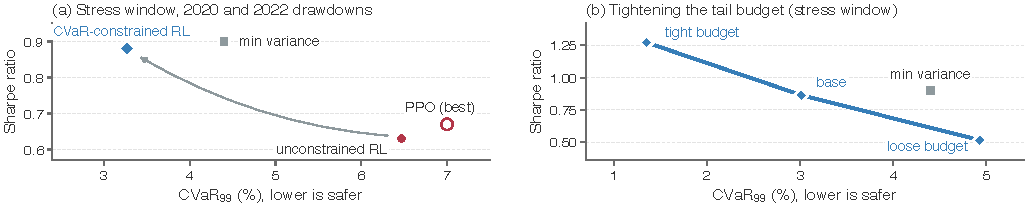
\includegraphics[width=\textwidth]{figure_cvar_hero.pdf}
  \Description{Two scatter plots of Sharpe ratio against CVaR99. On the left, the constrained allocator has higher Sharpe and lower CVaR99 on the stress window than the unconstrained allocator and PPO. On the right, moving from a loose to a tight tail budget raises Sharpe and lowers CVaR99 at each step, and the tight budget lies above and to the left of minimum variance.}
  \caption{(Left) Risk and return on the stress window for the unconstrained (circle) and constrained (diamond) allocators. (Right) Tightening the tail budget from loose to tight improves both CVaR$_{99}$ and Sharpe. The square marks minimum variance.}
  \label{fig:hero}
\end{figure*}

\subsection{Walk-forward across regimes (10 OOS folds, \texorpdfstring{$\approx$}{about }2010--2024)}
We refit every 52 weeks on a rolling 312-week window and concatenate 10 out-of-sample
folds. Out of sample, the constraint beats unconstrained RL on every metric, with Sharpe $+18\%$
(0.70\,$\to$\,0.83), $\mathrm{CVaR}_{99}$ $-20\%$ (0.0416\,$\to$\,0.0331) and max-DD $-25\%$
(15.1\%\,$\to$\,11.4\%). In absolute terms, inverse volatility (Sharpe 1.06, max-DD 0.070,
$\mathrm{CVaR}_{99}$ 0.0183) and minimum variance (1.45, 0.057, 0.0106) remain ahead, and minimum variance is the
strongest of all, so on this protocol the learner does not beat the
optimiser. On the
macro universe alone, the fold-level Wilcoxon on $\mathrm{CVaR}_{99}$ is marginal ($p=0.06$, with
5 of 10 folds improved), and the reduction concentrates in selloffs ($\mathrm{CVaR}_{99}$
$0.066\!\to\!0.048$, max-DD $0.218\!\to\!0.137$, Table~\ref{tab:regime}). A two-universe, 40-fold analysis raises the significance of the tail reduction to
$p=8.8\times10^{-6}$ (Section~\ref{sec:significance}).

\paragraph{When RL adds value, by regime}
The constrained policy does best relative to minimum variance in high-volatility periods
($n{=}71$), with Sharpe $2.169$ versus $1.668$ and CVaR$_{99}$ within $0.012$ of minimum variance's
floor. In calm markets ($n{=}388$) and selloffs ($n{=}61$), minimum variance dominates (selloff
Sharpe $0.035$ vs.\ constrained RL $-0.809$). The overlay adds value when volatility is
elevated but has not collapsed into a full drawdown, and stops adding value once liquidity
deteriorates. The constraint still cuts tail risk relative to unconstrained RL in all three
regimes ($-29.1\%$ calm, $-20.7\%$ high-vol, $-27.4\%$ selloff), which suggests that the
reduction comes from the pipeline and does not depend on the regime.\looseness=-1

\begin{table}[t]
\centering
\caption{Sharpe and CVaR$_{99}$ by regime, pooled from the 10-fold macro-ETF walk-forward ($n$ is the number of weeks in each regime).}
\label{tab:regime}
\footnotesize
\setlength{\tabcolsep}{2pt}
\begin{tabular}{lrrrrrr}
\toprule
 & \multicolumn{2}{c}{Calm ($n{=}388$)} & \multicolumn{2}{c}{High-vol ($n{=}71$)} & \multicolumn{2}{c}{Selloff ($n{=}61$)} \\
\cmidrule(lr){2-3}\cmidrule(lr){4-5}\cmidrule(lr){6-7}
Strategy & Sharpe & CVaR$_{99}$ & Sharpe & CVaR$_{99}$ & Sharpe & CVaR$_{99}$ \\
\midrule
RL Constrained   & 1.438 & 0.020 & 2.169 & 0.018 & $-0.809$ & 0.048 \\
RL Unconstrained & 1.282 & 0.028 & 2.194 & 0.023 & $-1.127$ & 0.066 \\
Min-Variance     & 1.770 & 0.009 & 1.668 & 0.007 & 0.035 & 0.016 \\
Inverse-Vol      & 1.721 & 0.011 & 2.803 & 0.009 & $-1.327$ & 0.033 \\
\bottomrule
\end{tabular}
\end{table}

\begin{table}[t]
\centering
\caption{Regime-switching hybrid against the pure strategies on the 26-week macro walk-forward, with bootstrap 95\% intervals from 50{,}000 resamples.}
\label{tab:hybrid}
\footnotesize
\begin{tabular}{lrrrr}
\toprule
Strategy & Sharpe & 95\% CI & Ann.\ Ret.\ & CVaR$_{99}$ \\
\midrule
Constrained RL (pure) & 0.942 & [0.29, 1.68] & 4.0\% & 0.025 \\
Min-variance (pure)   & 1.209 & [0.55, 1.93] & 2.9\% & 0.012 \\
Hybrid       & 1.316 & [0.66, 2.03] & 3.5\% & 0.013 \\
\bottomrule
\end{tabular}
\end{table}

\subsection{Statistical significance across two universes}
\label{sec:significance}
To check that the effect is not specific to one universe, we add the ten-sector universe
(Section~\ref{sec:data}) and shorten the walk-forward test fold to 26~weeks, which gives 20
folds per universe (Table~\ref{tab:stats}). Each universe shows a significant
fold-level reduction on its own, with macro-ETF Wilcoxon $p=0.0077$ (9 folds improved, 11 tied,
none worse) and sector $p=0.0003$ (17 improved, 2 tied, 1 worse), and
Benjamini--Hochberg~\cite{benjamini1995fdr} multiple-testing control rejects the null for
both. A tie is a fold
where the budget never binds, so the two learners coincide. The mean fold
$\Delta\mathrm{CVaR}_{99}$ is $-0.0041$ (macro-ETF) and $-0.0087$ (sector). Pooling all 40 folds
gives Wilcoxon $p=8.8\times10^{-6}$ and a bootstrap 95\,\% CI of $[-0.0089,\,-0.0041]$ on the
mean fold difference, and 26 of the 27 untied folds improve (sign test on directions only,
$p=4\times10^{-7}$).\looseness=-1

The two universes share a calendar, so their folds are not independent. We also average their differences within each calendar fold. The 20 resulting clusters give Wilcoxon
$p=3.3\times10^{-4}$ (exact sign-flip test $p=3.8\times10^{-5}$), and moving-block bootstrap intervals, which
resample runs of consecutive clusters to keep time order, exclude zero. The Probabilistic Sharpe Ratio~\cite{bailey2012sharpe} (the
probability that the true Sharpe is above zero) of the constrained allocator is $\geq 0.99$ on
both universes. Its out-of-sample Sharpe advantage
over classical baselines, however, does not survive the Deflated Sharpe
Ratio~\cite{bailey2014deflated}, which discounts a Sharpe ratio for the number of configurations
tried before reporting it. The significant effect is on tail risk, which is what a safety layer
is meant to deliver.\looseness=-1

\begin{table}[t]
\centering
\caption{Walk-forward CVaR$_{99}$ on two universes with 26-week folds. PSR is the Probabilistic Sharpe Ratio of the constrained allocator.}
\label{tab:stats}
\footnotesize
\setlength{\tabcolsep}{3pt}
\begin{tabular}{@{}lrrrrrr@{}}
\toprule
universe & folds & $\mathrm{CVaR}_{99}^{\text{unc}}$ & $\mathrm{CVaR}_{99}^{\text{con}}$ & improved & Wilcoxon $p$ & PSR \\
\midrule
macro ETF (7)   & 20 & 0.0143 & 0.0102 &  9/20 & 0.0077              & 0.997 \\
sector (10)     & 20 & 0.0336 & 0.0250 & 17/20 & 0.0003              & 0.990 \\
pooled & 40 & --- & --- & 26/40 & $8.8\times10^{-6}$ & --- \\
\bottomrule
\end{tabular}
\end{table}

\subsection{Generalisation to sector ETFs}
\label{sec:generalize}
Re-running the stress study unchanged on the ten-sector universe (mean over 3 seeds)
replicates the main effect. The constraint cuts $\mathrm{CVaR}_{99}$ by $30\%$
($0.109\!\to\!0.076$), $\mathrm{CVaR}_{95}$ by $35\%$ ($0.058\!\to\!0.037$), maximum drawdown by $30\%$
($0.295\!\to\!0.208$), and the breach rate by $47\%$ ($0.75\!\to\!0.40$), at
no Sharpe cost ($0.752\!\to\!0.748$). A paired block bootstrap of the
$\mathrm{CVaR}_{99}$ difference gives $-0.044$, with 95\% BCa interval
$[-0.050,\,-0.032]$ and $p\approx0$. The one difference from the macro universe is that
there the constraint improved Sharpe (the avoided tail losses outweighed the cost),
whereas on sectors it leaves Sharpe unchanged. The reduction in tail risk and drawdown
carries over to sectors.\looseness=-1

\subsection{Robustness and ablations}
The $\mathrm{CVaR}_{99}$ reduction holds in all 7 perturbations, even at
$3\times$ costs ($\mathrm{CVaR}_{99}$ 54\% lower, Sharpe 63\% above unconstrained).
Ablations show a consistent pattern (Figure~\ref{fig:hero}, right, with 3-seed means on the macro-ETF stress window). Tightening the tail budget from loose ($\alpha=0.95$, limit
$1.92\%$) through base ($1.2\%$) to tight ($\alpha=0.99$ or $0.72\%$) improves CVaR$_{99}$ and
Sharpe together at every step. The tightest configuration reaches Sharpe~$1.27$ and
CVaR$_{99}=1.4\%$, above minimum variance on the same window (Sharpe~0.90, CVaR$_{99}=4.4\%$)
and competitive with its walk-forward Sharpe of~1.45. Here tighter limits also raise return, which risk limits usually do not, because the constraint acts only on the worst weeks, through its tail-only gradient and tighter checkpoint selection, and so removes the
largest losses while leaving most of the return distribution unchanged. Against the base
configuration (Sharpe $0.865$, CVaR$_{99}$ $0.0301$, max-DD $0.111$), removing the anchor gives $0.826$, $0.0318$ and $0.108$, and $\alpha=0.90$ gives $0.684$, $0.0452$ and $0.172$. A Sharpe objective gives $0.791$, $0.0273$ and $0.108$, the loose budget $0.515$, $0.0493$ and $0.230$, $\alpha=0.99$ gives $1.251$, $0.0146$ and $0.053$, and the tighter budget $1.272$, $0.0135$ and $0.041$.\looseness=-1


\paragraph{Features} Rolling factor betas alone slightly hurt performance. Adding macro state
gives Sharpe $+0.02$ (3-seed mean) but worsens CVaR$_{99}$ ($0.029\!\to\!0.031$).\looseness=-1

\paragraph{Does the policy change its holdings?}
Three diagnostics show that the constraint changes what the policy holds, so the lower tail
metric is not a measurement artefact. The unconstrained allocator concentrates and holds through
the 2020 and 2022 drawdowns. The constrained one rotates into cash and rates and keeps a lower,
steadier rolling CVaR estimate. The tail control costs modestly higher turnover, with no
leverage or single-asset bets, and the policy stays long-only, diversified and within the
turnover cap.

\subsection{Tuned model-free RL remains weak}
\label{sec:modelfree}
We sweep 36 PPO and 8 SAC configurations, select each by validation Sharpe, and
evaluate on the stress window (Table~\ref{tab:modelfree}). Tuning does not help either family.
The selected PPO overfits validation (Sharpe $1.70$) and then has the worst out-of-sample
tail (Sharpe $0.67$, $\mathrm{CVaR}_{99}=0.070$), while SAC collapses to near-zero turnover
(Sharpe $0.39$). With 887 weekly observations, score-function and
off-policy RL have too few effective samples. The constrained allocator matches minimum
variance on Sharpe ($0.91$ vs $0.90$) and lowers $\mathrm{CVaR}_{99}$ by $27\%$ ($0.032$ vs
$0.044$).

\begin{table}[t]
\centering
\caption{Best-tuned model-free RL (selected on validation Sharpe, 3-seed mean) against the differentiable allocators and minimum variance on the stress window.}
\label{tab:modelfree}
\footnotesize
\begin{tabular}{lrrrr}
\toprule
strategy & Sharpe ($\uparrow$) & $\mathrm{CVaR}_{99}$ ($\downarrow$) & max-DD ($\downarrow$) & turnover ($\downarrow$) \\
\midrule
minimum variance        & 0.90 & 0.044 & 0.113 & 0.011 \\
diff.\ constrained & 0.91 & 0.032 & 0.113 & 0.039 \\
diff.\ unconstrained    & 0.60 & 0.062 & 0.212 & 0.023 \\
PPO (best)              & 0.67 & 0.070 & 0.225 & 0.028 \\
PPO (best) + CVaR       & 0.63 & 0.047 & 0.160 & 0.162 \\
SAC (best)              & 0.39 & 0.033 & 0.185 & 0.005 \\
SAC (best) + CVaR       & 0.18 & 0.035 & 0.205 & 0.004 \\
\bottomrule
\end{tabular}
\end{table}

\subsection{Evaluation-protocol reversal}
\label{sec:protocol}
To test how much the choice of evaluation protocol alone can change the conclusions, we
use the 31-asset universe (Section~\ref{sec:data}). Covariance estimation is harder here, so a learner has, in principle, more
room to add value. On a single stress split (train pre-2018, test through 2024), the constrained
learner appears to beat every optimiser, with Sharpe $0.85$ against $0.23$ for minimum
variance (Table~\ref{tab:protocol}). Under a rolling walk-forward (20 out-of-sample folds, refit
every 26 weeks), the same minimum-variance optimiser is instead the best method by a
wide margin, with Sharpe $1.40$ against the learner's $0.74$, so the ranking inverts.

The stress-split result depends on one fixed period and disappears under rolling refits.
Covariance shrinkage does not explain it. On the same split, Ledoit--Wolf minimum
variance~\cite{ledoit2004wellconditioned} reaches Sharpe $0.25$ and the min-CVaR LP $0.26$. The
tail-risk effect holds under both protocols (the constraint still lowers $\mathrm{CVaR}_{99}$
against the unconstrained learner fold by fold, Wilcoxon $p=6\times10^{-4}$), while the apparent
advantage over the optimiser does not. We recommend rolling walk-forward with
Deflated-Sharpe~\cite{bailey2014deflated} as the reporting standard, and treat single
stress-window comparisons of learned allocators against optimisers as unreliable.\looseness=-1

\begin{table}[t]
\centering
\caption{Sharpe ratios by protocol, same 31-asset universe.}
\label{tab:protocol}
\footnotesize
\setlength{\tabcolsep}{3.5pt}
\begin{tabular}{@{}lrrrr@{}}
\toprule
protocol & min-var & inv-vol & constr.\ (ours) & unconstr. \\
\midrule
stress split       & 0.23 & 0.38 & 0.85 & 0.70 \\
walk-forward (OOS) & 1.40 & 0.78 & 0.74 & 0.56 \\
\bottomrule
\end{tabular}
\end{table}


%% =====================================================================
\section{Discussion}
\label{sec:discussion}

\paragraph{How close is the learner to minimum variance?} It depends on the arm. The
unfiltered learner is far from it. Its mean per-rebalance $L_1$ weight distance to the
rolling min-variance path is $0.89$ (of a maximum $2.0$), with correlation $0.20$ and a
different top-weighted asset in $97\%$ of weeks. The similarity suggested by the tightest
ablation (Figure~\ref{fig:hero}, right) is in aggregate risk statistics and does not
extend to holdings. The filtered arms are closer ($L_1$ $0.48$ to $0.61$, correlation $0.72$ to
$0.79$). They achieve compliance partly by holding low-volatility portfolios, and from there
they improve on minimum variance in breach depth, and A5 also in Sharpe
(Section~\ref{sec:coupling}).\looseness=-1

We draw three practical lessons. First, tail limits reduce risk before a crash, as the constrained allocator moved to cash two weeks before the COVID trough (drawdown $7.7\%$ against
$16.3\%$ unconstrained in March 2020). Second, the constraint is most useful as an overlay in high-volatility
periods (Table~\ref{tab:hybrid}). Third, a multiplier stuck near zero means the constraint is inactive, so check the coupling and use out-of-sample folds before claiming an edge over an
optimiser.\looseness=-1

%% =====================================================================
\section{Scope}
\label{sec:limitations}
The pure learned allocator does not beat rolling minimum variance on Sharpe out of sample, a
Deflated-Sharpe correction removes its apparent Sharpe edge over classical baselines, and the
hybrid's $+0.107$ gain comes only from high-volatility weeks. The study covers two
equity-centric universes at weekly frequency with proportional costs (no market impact or
borrow), the macro features are lagged for availability but are not vintage data, and the
protocol reversal is shown on a single 31-asset window. The filter's Gaussian CVaR estimate can
understate fat-tailed losses, and the constrained learner trails minimum variance in selloff
weeks (Table~\ref{tab:regime}). Within these limits, the paper contributes a tail-risk safety
layer for learned allocators and evaluation lessons that transfer to other constrained RL
studies in finance.\looseness=-1

\section{Conclusion and future work}
\label{sec:conclusion}

Our differentiable CVaR-constrained allocator consistently reduces tail risk (26 of 27 untied
folds, $p=8.8\!\times\!10^{-6}$), removes portfolio-constraint violations under stress and
reduces risk before crisis troughs, and a regime-switching hybrid reaches Sharpe $1.316$
against $1.209$ for min-variance (with overlapping intervals). We describe two failure modes
that apply to constrained RL in finance generally, a Lagrangian constraint-coupling
failure and an evaluation-protocol reversal, and show that a decision-time CVaR filter
achieves the out-of-sample compliance that neither rescaling the dual nor recalibrating the
budget achieved. Constrained RL is best used as a safety layer and an overlay for
high-volatility periods. Its lasting benefits are lower tail risk and compliance with the
budget.\looseness=-1

\bibliographystyle{ACM-Reference-Format}
\bibliography{references}

\end{document}
